% \documentclass[%
%  reprint,
% %superscriptaddress,
% %groupedaddress,
% %unsortedaddress,
% %runinaddress,
% %frontmatterverbose, 
% %preprint,
% %preprintnumbers,
% %nofootinbib,
% %nobibnotes,
% %bibnotes,
% %amsmath,amssymb,
%  aps,
% %pra,
% %prb,
% %rmp,
% %prstab,
% %prstper,
% %floatfix, 
% 10pt,
% conference
% ]{IEEEtran}
\documentclass[conference]{IEEEtran}


\usepackage{IEEEtrantools}

\usepackage{graphicx} % Required for inserting images
\usepackage{amsfonts} % for "\mathbb" macro
\usepackage{amsmath}
\usepackage{amssymb}
\usepackage{amsthm}
\usepackage{mathtools}
\usepackage{braket}
\usepackage{tikz}
\usepackage{algpseudocode}
\usepackage{algorithm}
\usepackage{float}
\usepackage{caption}
\usepackage[sort&compress,numbers]{natbib}
\usepackage{hyperref}
\usepackage[T1]{fontenc}

\DeclareCaptionFormat{algor}{%
  \hrulefill\par\offinterlineskip\vskip1pt%
    \textbf{#1#2}#3\offinterlineskip\hrulefill}
\DeclareCaptionStyle{algori}{singlelinecheck=off,format=algor,labelsep=space}
\captionsetup[algorithm]{style=algori}

\usepackage{etoolbox}\AtBeginEnvironment{algorithmic}{\small} 



\newtheorem{theorem}{Theorem}
\newtheorem{result}{Result}
\newtheorem{corollary}[theorem]{Corollary}
\newtheorem{remark}[theorem]{Remark}
\newtheorem{lemma}[theorem]{Lemma}
%\newtheorem{observation}[theorem]{Observation}
%\newtheorem{proposition}[theorem]{Proposition}
\newtheorem{definition}[theorem]{Definition}
%\newtheorem{claim}[theorem]{Claim}
%\newtheorem{fact}[theorem]{Fact}
%\newtheorem{assumption}[theorem]{Assumption}
\newtheorem{example}{Example}

\newenvironment{example*}
  {\addtocounter{example}{-1}\example}
  {\endexample}

%\newtheorem*{theorem*}{Theorem}
%\newtheorem*{corollary*}{Corollary}
%\newtheorem*{lemma*}{Lemma}
%\newtheorem*{proposition*}{Proposition}
%\newtheorem*{definition*}{Definition}
%\newtheorem*{example*}{Example}
%\newtheorem*{remark*}{Remark}
%\newtheorem*{problem*}{Problem}


\newcommand{\llbr}{[\![}
\newcommand{\rrbr}{]\!]}
\newcommand{\nr}[1]{{\color{blue} #1}}


\begin{document}


%\title{G-Hatchet: An Algorithm for Decomposing Stabilizers \\ into Lower Weight Gauge Operators}
%\title{G-Hatchet: Splitting Stabilizers into Gauges}
\title{GNarsil: Splitting Stabilizers into Gauges}
\makeatletter
\newcommand{\linebreakand}{%
  \end{@IEEEauthorhalign}
  \hfill\mbox{}\par
  \mbox{}\hfill\begin{@IEEEauthorhalign}
}
\makeatother

\author{
  \IEEEauthorblockN{Oskar Novak}
  \IEEEauthorblockA{\textit{Wyant College of Optical Sciences} \\
    \textit{University of Arizona}\\
    Tucson, USA \\
    onovak@arizona.edu}
  \and
  \IEEEauthorblockN{Narayanan Rengaswamy}
  \IEEEauthorblockA{\textit{Department of Electrical and Computer Engineering} \\
    \textit{University of Arizona}\\
    Tucson, USA \\
    narayananr@arizona.edu}
}


% \date{\today}                    


\maketitle
% \IEEEdisplaynontitleabstractindextext


\begin{abstract}

Quantum subsystem codes have been shown to improve code performance, ease the implementation of logical operations on codes, and make measuring stabilizers easier by decomposing them into smaller weight gauge operators. In this paper, we present a set of algorithms that facilitate decomposing stabilizers of a given CSS code into smaller weight gauge operators compatible with the current stabilizers and logical operators of the code. We also provide novel examples of new subsystem codes that outperform current versions of them in this regard, such as the SLP construction. Finally, based on our experiments, we share some general insights about non-locality's effects on stabilizer decomposition performance.
\end{abstract}


\section{Introduction}


\IEEEPARstart{Q}{uantum} error correction is vital for quantum computers to achieve their full potential. 
This requires identifying the location of errors on a quantum computer without disturbing the delicate superposition states of the qubits involved in the computation. 
This is done by measuring stabilizers, which can help elucidate where the errors are located through an error syndrome. 
However, measuring these stabilizers is a nontrivial task: if measuring the stabilizers requires measuring a high number of qubits, this process poses the risk of creating additional errors.

Subsystem codes may help alleviate this issue. 
These are codes with gauge operators or operators on qubits that do not carry quantum information. %These gauge operators can give the same information as a higher-weight stabilizer by taking the product of each of their eigenvalues together. 
If designed well, then the eigenvalue of a high-weight stabilizer can be obtained as a product of the eigenvalues of several lower-weight gauge operators that can be measured more easily.
Generally, these gauge operators form a non-abelian group, meaning that the order of measurement matters. 
This is dealt with by a process called gauge fixing, where changes to the code can be made mid-computation to help ease measuring stabilizers or even implementing logical operations~\cite{nbreuckmann}. 
There are several examples of subsystem codes in the literature. 
Most have nice geometrically local properties, which makes finding the gauge group an intuitive process~\cite{higgott2021subsystem}. 
Closed-form expressions exist for constructing generalized Bravyi-Bacon-Shor or Subsystem Hypergraph Product (SHP) Codes~\cite{li2020numerical}. 
There are also some computational methods for forming a set of gauge generators out of a set of Pauli operators via Gram-Schmidt orthogonalization \cite{wilde2009logical}, and computational search methods for finding a gauge code from a set of two-qubit measurement operators~\cite{crosswhite2011automated}. 
Some papers have even translated these gauge-fixing insights of subsystem codes into the ZX calculus \cite{huang2023graphical}.  

However, no algorithm allows one to take a stabilizer code and find a subsystem code directly from it, especially one that finds the gauge operators whose product is (most of) a stabilizer. 
We present a set of algorithms capable of doing this for CSS stabilizer codes and present non-trivial examples of subsystem codes found by our algorithms. 
In particular, we demonstrate a modified Subsystem Hypergraph Product (SHP) code that has gauge operators that multiply to most of a stabilizer generator but whose leftover gauge operators needed to measure the entire stabilizer are lower weight than those obtained from the closed-form expressions in~\cite{li2020numerical}, and an extension to the SHP code called the Subsystem Lifted-Product code (SLP), which can have superior performance to a typical Lifted Product code built out of the same Base Matrix.

%gauge operators to do the same thing.




\section{Background}




\subsection{Representing Pauli Operators as  Binary Vectors}
Given the vectors $ a=[a_{1},...,a_{n}]$, $ b=[b_{1},...,b_{n}]\in \mathbb{F}^{n}_{2}$, we define the Hermitian operator
\begin{equation}
    E(a,b) \coloneqq i^{a_{1}b_{1}}X^{a_{1}}Z^{b_{1}}\otimes...\otimes i^{a_{n}b_{n}}X^{a_{n}}Z^{b_{n}}, 
\end{equation}
where $X$ and $Z$ are the standard Pauli operators and $i \coloneqq \sqrt{-1}$.
We can define the $n$-qubit Pauli group $\mathcal{P}_{n}$ as
\begin{equation}
\begin{aligned}
    \mathcal{P}_{n} \coloneqq \left< i^{\alpha} E(a,b)\ | \ a,b \in \mathbb{F}^{n}_{2}; \alpha \in \{0,1,2,3\} \right>.
\end{aligned}
\end{equation}
This is also known as the Heisenberg-Weyl Group $HW_{N}, \ N=2^{n}$. 
The standard symplectic inner product in $\mathbb{F}^{2n}_{2}$ is defined as \cite{rengaswamy2018synthesis}:
\begin{align}
\left<[a,b],[a',b']\right>_{s} & \coloneqq a'b^{T}+b'a^{T} \ (\mathrm{mod} \ 2) \nonumber \\
%
\label{eq:symp_inn_pdt}
  &= [a,b]\ \mathrm{\boldsymbol{\Omega}}\ [a',b']^{T} \ (\mathrm{mod} \ 2),
\end{align}
where the matrix $\boldsymbol{\Omega}=\begin{bmatrix} 
  \boldsymbol{0} & \boldsymbol{I}_n \\
  \boldsymbol{I}_n & \boldsymbol{0}
  \end{bmatrix}$ is the symplectic form in $\mathbb{F}^{2n}_{2}$.
We notice that two operators  $E(a,b)$, $E(a',b')$ commute if and only if $\left<[a,b],[a',b']\right>_{s} =0$ (mod 2). Thus, we see that a vector $[a,b] \in \mathbb{F}^{2n}_{2} $ is isomorphic to an operator $E(a,b)$ via the map $\gamma: \mathcal{P}_{n}/\left<i^{\alpha} \boldsymbol{I}_{2^n}\right> \xrightarrow{} \mathbb{F}^{2n}_{2}$ defined by
\begin{equation}
\gamma(E(a,b)) \coloneqq [a,b].
\end{equation}
Thus, without loss of generality, we can represent $n$ qubit Pauli operators as binary vectors throughout this paper. 
The \textit{weight} of an $n$-qubit Pauli operator is the number of qubits on which it applies a non-identity Pauli operator.
For example, the operator $X_{1}\otimes X_{2} \otimes I_{3}$ can be described as $\begin{bmatrix} 1 & 1 & 0, & 0 & 0 & 0 \end{bmatrix}$, and its weight is $2$.



\subsection{Quantum Stabilizer Codes}



A stabilizer group $\mathcal{S}\in \mathcal{P}_{n}$ is an abelian subgroup of the Pauli group that does not contain $-I$. 
The corresponding \textit{stabilizer code} is defined by: 
\begin{equation} 
\mathcal{Q} \coloneqq \left\{ \ket{\psi} \in \mathbb{C}^{2^n} \colon S\ket{\psi}=\ket{\psi} \ \forall\ S \in \mathcal{S} \right\}.
\end{equation} 
%A quantum code with a code space $\mathcal{C}$ defined in this manner is a \textit{quantum stabilizer code}. 
A stabilizer code with $n$ physical qubits and $m$ stabilizer generators can encode $k=n-m$ logical qubits. The logical operators of the code come from the centralizer of $\mathcal{S}$, defined as
%denoted $\mathcal{C}(\mathcal{S})$, where 
\begin{equation}
\mathcal{C}(\mathcal{S}) \coloneqq \left\{ U\in \mathcal{P}_{n} \colon [U,S]=0 \ \forall\ S \in \mathcal{S} \right\},
\end{equation}
where $[U,S] \coloneqq US - SU$ is the commutator of $U$ and $S$.
Here, notice that $\mathcal{S} \subset \mathcal{C}(\mathcal{S})$. 
Finally, the \textit{minimum distance}, $d$, of the code is given by the minimum weight of any Pauli operator in $\mathcal{C}(\mathcal{S}) \setminus \mathcal{S}$, or the lowest weight logical operator. 
Thus, we denote the parameters of a quantum stabilizer code as $\llbr n,k,d \rrbr$. Finally, a CSS code is a stabilizer code whose stabilizer $\mathcal{S}=\left< \gamma^{-1}(\boldsymbol{H}_{X}),\gamma^{-1}(\boldsymbol{H}_{Z})\right>$, $\boldsymbol{H}_{X}\boldsymbol{H}_{Z}^{T}=\boldsymbol{0}$, where $\boldsymbol{H}_{X}$, $\boldsymbol{H}_{Z}$ are classical binary parity check matrices, and the map $\gamma^{-1}$ is applied to each row of $\boldsymbol{H}_{X}$, $\boldsymbol{H}_{Z}$.



\subsection{Subsystem Codes}



A subsystem code is a quantum error-correcting code that splits the code space $\mathcal{C}=A\otimes B$ into the logical subspace, $A$, and a gauge subspace, $B$, that does not carry any logical information~\cite{nbreuckmann}. Thus, the Hilbert space of a subsystem code can be written as $\mathcal{H}=\mathcal{C} \oplus \mathcal{C}^{\perp}=A \otimes B \oplus \mathcal{C}^{\perp}$. The gauge subspace is supported on $r$ gauge qubits, such that given $n$ physical qubits, $m$ stabilizers, and $r$ gauge qubits, the number of logical qubits is $k=n-m-r$.  Thus, a subsystem code with these parameters can be written as an $ \llbr n,k,r,d \rrbr$ subsystem code with code distance $d$. A subsystem code is defined by its gauge group 
\begin{equation}
    \mathcal{G} \coloneqq \left< iI,\mathcal{S},X_{1}',Z_{1}', \ldots, X_{r}',Z_{r}' \right> \subset \mathcal{P}_{n},
\end{equation} 
where $X_{i}', Z_{i}'$ are the  Pauli  operators for the $i$th gauge qubit, and $\mathcal{S}$ is the stabilizer group of the code. 

We can use $\mathcal{G}$ to define the stabilizers of the code: 
\begin{equation}
    \mathcal{S}\coloneqq\mathcal{Z}(\mathcal{G})=\mathcal{C}(\mathcal{G}) \cap \mathcal{G},
\end{equation} 
where $\mathcal{Z}(\mathcal{G})$ is the center of $\mathcal{G}$, and  $\mathcal{C}(\mathcal{G})$ is the centralizer of $\mathcal{G}$. We also define the bare logical operators $\mathcal{L}_{b}$ as: 
\begin{equation}
\mathcal{L}_{b}\coloneqq\mathcal{C}(\mathcal{G}) \setminus \mathcal{G} = \mathcal{C}(\mathcal{G}) \setminus \mathcal{S}.
\end{equation} 
These are the $k$ pairs of anti-commuting operators such that $[\mathcal{G},\mathcal{L}_b]=0$. These operators only act non-trivially on the subspace $A$. We also have the dressed logical operators $\mathcal{L}$, $\mathcal{L}_{b} \subset \mathcal{L}$, where: 
\begin{equation} 
\mathcal{L}=\mathcal{C}(\mathcal{S}) \setminus \left< i\mathcal{I} \right>. 
\end{equation} 
In other words, the set of dressed logical operators is the set of bare logical operators multiplied by an operator from $\mathcal{G} \setminus \left< i\mathcal{I} \right>$.

\begin{figure}[h]
 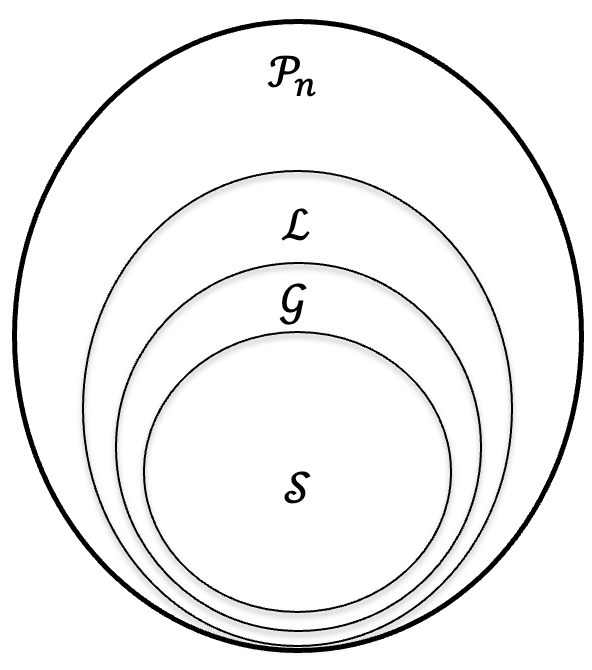
\includegraphics[scale=0.3]{vennd.png}
\centering
\caption{A diagram describing the relation of the Gauge group $\mathcal{G}$ to the other important subsets of $\mathcal{P}_{n}$ for constructing a subsystem code.}
\end{figure}



Finally, we can find the code distance $d$ such that 
\begin{equation}
    d \coloneqq \underset{P \in \mathcal{L}}{\min}\ |P|,
\end{equation} 
i.e., the minimum weight of a dressed logical operator.



\section{Describing Subsystem Codes via Binary Matrices}
\subsection{Stabilizer Code Construction via Binary Matrices}
We can describe a stabilizer code as a $2n \times 2n$ matrix $\boldsymbol{U}$ which has the following form \cite{rengaswamy2018synthesis}:
\begin{equation} 
\label{eq:U_matrix}
\boldsymbol{U}=
\begin{bmatrix}
    \mathcal{L}_{X} \\
    \mathcal{S} \\
    \mathcal{L}_{Z} \\
    \mathcal{S}'
\end{bmatrix}
\end{equation}
where its rows $\left<\boldsymbol{u}_{1},...,\boldsymbol{u}_{2n}\right>$ span $\mathbb{F}^{2n}_{2}$. 
We are overloading notation to represent both the group as well a binary matrix whose rows represent the generators of the group.
Here, $\mathcal{L}_{X}$ and  $\mathcal{L}_{Z}$ are the binary matrices that represent the generators of the logical Pauli operators. 
The sub-matrix $\mathcal{S}'$, otherwise known as the ``destabilizer''~\cite{Aaronson-pra04}, is added so that $\boldsymbol{U}$ has full rank. For a stabilizer code, we choose $\mathcal{S}'$ such that:
\begin{equation}
\label{eq:U_condition}
\boldsymbol{U}\boldsymbol{\Omega}\boldsymbol{U}^T=\boldsymbol{\Omega} \ (\mathrm{mod} \ 2).
\end{equation}
This means that each row vector in $\mathcal{S}'$ is chosen so that it anti-commutes with only one stabilizer generator inside $\mathcal{S}$. 
In other words, $\boldsymbol{U}$ is a binary symplectic matrix~\cite{Dehaene-pra03}.

\begin{theorem} 
Let $\boldsymbol{U}$ be a $2n \times 2n$ binary matrix constructed as in~\eqref{eq:U_matrix}. 
If $\boldsymbol{U}$ satisfies~\eqref{eq:U_condition}, then $\boldsymbol{U}$ describes a valid stabilizer code.
\begin{proof}
The L.H.S. of~\eqref{eq:U_condition} is our definition of the symplectic inner product in~\eqref{eq:symp_inn_pdt} extended to a matrix. 
Since $\boldsymbol{\Omega}$ has a single non-zero element per row, each row of $\boldsymbol{U}$ anti-commutes with exactly one other row, which is $n$ rows below (or above) it. 
Such pairs of rows are called \textit{symplectic pairs}.
Since an $ \llbr n,k,d \rrbr$ stabilizer code 
has $n-k$ stabilizers, the symplectic pairs of rows in $\mathcal{L}_{X}$ must be in the rows of $\mathcal{L}_{Z}$. This means that the codes' logical operators represented as binary vectors commute with the operators represented as binary vectors in $\mathcal{S}$, $\mathcal{S}'$. 

Thus, satisfying~\eqref{eq:U_condition} verifies all necessary conditions for $\boldsymbol{U}$ to represent a valid stabilizer code.
\end{proof}
\end{theorem}


\subsection{Subsystem Code Construction via Binary Matrices}



To construct a subsystem code using the methods of the previous section, we can take a binary matrix $\boldsymbol{U}$ constructed as in \eqref{eq:U_condition}, and choose $2r$ rows of it to become our gauge generators, and $\mathcal{L}_{X}$, $\mathcal{L}_{Z}$ become our bare logical operators. 

It should be noted that, generally, one can replace these $2r$ rows with other rows and still have a valid subsystem code, as long as $\boldsymbol{U}$ remains symplectic. 
Also, one is free to choose logical operators to become gauge operators. 
Thus, we state the following theorem: 

\begin{theorem} 
Let $\boldsymbol{U}$ be a $2n \times 2n$ binary matrix that has the construction of  \eqref{eq:U_condition} except that  $2r$ of its rows have possibly been altered. We call this altered matrix $\boldsymbol{U}'$. 
Then $\boldsymbol{U}'$ represents a valid subsystem code if:
\begin{equation}
\label{eq:U'_matrix}\boldsymbol{U'}\boldsymbol{\Omega}\boldsymbol{U}'^T=\boldsymbol{\Omega} \ (\mathrm{mod} \ 2).
\end{equation}
\begin{proof}
Since only the $2r$ rows that have been altered are those promoted to gauge operators, the rest of the rows of the matrix on the R.H.S. of \eqref{eq:U'_matrix} are identical to the rows in the same positions in \eqref{eq:U_condition}. This means the bare logical operators only anti-commute with their respective symplectic pairs and commute with the operators that generate the gauge group. Furthermore, this also means that since the leftover stabilizers in $\mathcal{S}$ only anti-commute with the leftover operators in $\mathcal{S}'$, the operators of $\mathcal{S}=\mathcal{Z}(\mathcal{G})$. Finally, as long as the previous conditions are met, then \eqref{eq:U'_matrix} guarantees that $\boldsymbol{U}'$ represents a valid subsystem code.
\end{proof}

\end{theorem}
A proof detailing our algorithm's ability to find all suitable representations for the gauge generators is included in Appendix A.




\section{Using Binary Matrix Methods to Find Useful Gauge Operators}


Here we will use \textit{gauge generators} to describe the non-stabilizer generators of the gauge group.
In practice, a subsystem code's utility comes from measuring the product of a set of lower-weight gauge operators that yields the same information as measuring a higher-weight stabilizer \cite{higgott2021subsystem}. 
Using the binary matrix constructions of the previous section, we can find low-weight gauge operators for CSS codes whose composition produces the code's stabilizers up to a remaining gauge operator that is not a gauge generator.
Let us call this remaining gauge operator the \emph{residual operator} for that stabilizer.
We refer to the minimum (Pauli) weight over all residual operators as the \textit{residual weight}.
For a gauge decomposition to be useful, the residual weight must be less than the weight of the decomposed stabilizer. 
To achieve this, we propose two algorithms. 
The first algorithm finds the set of $r$ gauge generators that decompose stabilizers with the least residual weight and then adds back stabilizers so that $n=k-r-m$ is still satisfied.  
We describe the first \emph{GNarsil} algorithm, which ``cuts'' stabilizers into gauges, in Algorithm \ref{alg:euclid}.

% \begin{algorithm}[H]
% % \captionof{algorithm}{Method for Finding Suitable Gauge Generators }\label{euclid}
% \caption{Method for Finding Suitable Gauge Generators}
% \label{alg:euclid}

% \begin{algorithmic}[2]
% \Require $\boldsymbol{U} \gets 
% \begin{bmatrix}
%     \mathcal{L}_{X} \\
%     \mathcal{S} \\
%     \mathcal{L}_{Z}\\
%     \mathcal{S'}
% \end{bmatrix}$, $G_{XrowIndeces} \gets$ indices of $\boldsymbol{U}$ $1:r$,\\$G_{ZrowIndeces} \gets$ indices of $\boldsymbol{U}$ $(r+1):(2r)$,\\$\mathrm{weight} \gets gaugeWeight$,\\$\mathrm{maxSize} \gets s$,\\$S_{Xtargets} \gets$ indices of $\boldsymbol{U}$ corresponding to $X$ stabilizers to split,\\$S_{Ztargets} \gets$ indices of $\boldsymbol{U}$ corresponding to $Z$ stabilizers to split, \\
% $\mathrm{gaugesPerStab} \gets m$
  
 
 
% \\
%   \State  assign $X$ops  all $X$ bit strings with weight $w$ and length $2n$
%    \State  assign $Z$ops  all $Z$ bit strings with weight $w$ and length $2n$
 
%   \\
%   \Comment{Find X,Z Gauges }
%    \State $\boldsymbol{V}\gets \boldsymbol{U}-\mathcal{S'}$
%   \For{$i$ in 1:size($X\mathrm{ops}$,$Z\mathrm{ops}$)}
  
%   \If{$\left<X\mathrm{ops}\left(i\right),Z\mathrm{ops}\left(i\right),\boldsymbol{V}\right>_{s}=\boldsymbol{0}$\ (mod 2)}
%   \If{$\mathrm{rank}\left(\begin{bmatrix}
%       \boldsymbol{V}\\
%       X\mathrm{ops}\left(i\right),Z\mathrm{ops}\left(i\right)
%   \end{bmatrix}\right)>\mathrm{rank}\left(\boldsymbol{V}\right)$}
%   \If{$\mathrm{rank}\left(\begin{bmatrix}
%       \mathrm{valid}X\mathrm{Gauges},\mathrm{valid}Z\mathrm{Gauges}\\
%       X\mathrm{ops}\left(i\right),Z\mathrm{ops}\left(i\right)
%   \end{bmatrix}\right)>\mathrm{rank}\left(\mathrm{valid}X\mathrm{Gauges},\mathrm{valid}Z\mathrm{Gauges}\right)$}
  
%   \If{ operatorWeight$\left(\left<Z\mathrm{ops}\left(i\right),\mathcal{G}_{X}\right>_{s}\right) = 1$\  or an $X$ operator}
%   \State $ \mathrm{valid}X\mathrm{Gauges},\mathrm{valid}Z\mathrm{Gauges} \gets X\mathrm{ops}\left(i\right),Z\mathrm{ops}\left(i\right)$ 
%   \EndIf
%   \EndIf
%   \EndIf
%   \EndIf
%   \If{size(validX,Zgauges) $\geq$ maxSize}
%  \State \textbf{break}
%   \EndIf
  
%   \EndFor
% \If{$\mathrm{valid}X\mathrm{Gauges},\mathrm{valid}Z\mathrm{Gauges}$ is empty}
% \State weight $\gets$ weight $+ \ 1$
% \State \textbf{go} to 12
% \EndIf
% \State $X\mathrm{gChoices},Z\mathrm{gChoices} \gets $

% $\mathrm{allCombs}\left(\mathrm{size}\left(\mathrm{valid}X\mathrm{Gauges},\mathrm{valid}Z\mathrm{Gauges}\right),\mathrm{gaugesPerStab}\right)$
% \If{weight $\geq$ n}
%  \State \textbf{stop}
%  \Comment{Algorithm Fails}
% \EndIf
% \For{$i$ in $\mathcal{S}_{Xtargets},\mathcal{S}_{Ztargets}$}
% \For{$j$ in  1:size($X\mathrm{gChoices},Z\mathrm{gChoices}$)}
% \State resultantGauge $\gets \textbf{sum} \boldsymbol{U}(i)+\boldsymbol{U}\left(X\mathrm{gChoices}\left(j\right),Z\mathrm{gChoices}\left(j\right)\right)$ (mod 2)
% \State residualWeight $\gets$ operatorWeight(resultantGauge)
% \EndFor
% \\
% \textbf{sort}  residualWeight
% \State $\mathcal{G}_{X,Z} \gets$ validX,Zgauges \textbf{with} smallest residualWeight
% \For{$j$ in  1:size($X\mathrm{gChoices},Z\mathrm{gChoices}$)}
% \If{$\mathcal{G}_{X,Z}$ contains operators in $X\mathrm{gChoices}\left(j\right),Z\mathrm{gChoices}\left(j\right)$}
% \State \textbf{remove} $X\mathrm{gChoices}\left(j\right),Z\mathrm{gChoices}\left(j\right)$  \textbf{from}
% $X\mathrm{gChoices},Z\mathrm{gChoices}$
% \EndIf
% \EndFor
% \EndFor
% \State \textbf{go} to 12 when done with X case

% \State replace unused Stabilizers in $\mathcal{S'}$ 
% \State \textbf{Output:} $\boldsymbol{U}$, codeDistance($\boldsymbol{U}$)

% \end{algorithmic}
% \end{algorithm}



\begin{algorithm}
% \captionof{algorithm}{Method for Finding Suitable Gauge Generators }\label{euclid}
\caption{GNarsil 1: Gauge Generators to Split Stabilizers}
\label{alg:euclid}

\begin{algorithmic}[1]


\State \textbf{Input:} $\boldsymbol{U} = 
\begin{bmatrix}
    \mathcal{L}_{X} \\
    \mathcal{S} \\
    \mathcal{L}_{Z}\\
    \mathcal{S'}
\end{bmatrix}$, $\{ i_1, i_2, \ldots, i_r \} \subseteq \{ k+1, k+2, \ldots, n \}:$ indices of rows of $\boldsymbol{U}$ to be replaced with $X$-type gauge generators, desired Pauli weight $w$ for gauge generators

\State \textbf{Initialization:} 

% $G_{\rm XrowIndices} \gets \{ i_1, i_2, \ldots, i_r \}$; 

% $G_{\rm ZrowIndices} \gets \{ n+i_1, n+i_2, \ldots, n+i_r \}$; 

$\mathcal{G}_X \gets \emptyset, \ \mathcal{G}_Z \gets \emptyset$

$\mathrm{validXGauges} \gets \emptyset, \ \mathrm{validZGauges} \gets \emptyset$

% $\mathrm{XresidualWeight} \gets n, \ \mathrm{XresidualWeight} \gets n$

% $\mathrm{weight} \gets w$; 

$\mathrm{maxSize} \gets $ max. number of gauge candidates to consider; 

$S_{\rm Xtargets} \gets$ indices of rows of $\boldsymbol{U}$ that are $X$-stabilizers; 

$S_{\rm Ztargets} \gets$ indices of rows of $\boldsymbol{U}$ that are $Z$-stabilizers; 

$\mathrm{gaugesPerStab} \gets $ \# of gauge generators per stabilizer; 

Xops $\gets$ weight-$w$ vectors in $\{0,1\}^{n}$ appended with $\boldsymbol{0}$ at\\ \hspace{1.75cm} the end to make length $2n$ (for $X$-gauges); 

Zops $\gets$ weight-$w$ vectors in $\{0,1\}^{n}$ appended with $\boldsymbol{0}$ at\\ \hspace{1.75cm} the beginning to make length $2n$ (for $Z$-gauges); 

$\boldsymbol{V}\gets \boldsymbol{U}(1:(n+k))$ (i.e., remove $\mathcal{S}'$ from $\boldsymbol{U}$) 

\Comment{Find $X$, $Z$ gauge generators}

\For{$i$ in 1:size($X\mathrm{ops}$)}
  
  \If{size(validXGauges) $\geq$ maxSize}
  \State \textbf{break}
  \EndIf
  
  \If{$\langle \mathrm{Xops}(i), \boldsymbol{V} \rangle_{s} = \boldsymbol{0}\ (\bmod\ 2)$ and \\%
      \hspace{7mm} $\mathrm{rank}\left(
      \begin{bmatrix}
      \boldsymbol{V}\\
      \mathrm{Xops}(i)
      \end{bmatrix} \right) > \mathrm{rank}(\boldsymbol{V})$ and \\%
      \hspace{7mm} $\mathrm{rank}\left(
      \begin{bmatrix}
      \mathrm{validXGauges}\\
      \mathrm{Xops}(i)
      \end{bmatrix} \right) > \mathrm{rank}\left( \mathrm{validXGauges} \right)$ and \\%
      \hspace{7mm} size(validXGauges) $<$ maxSize}
      
   \State $\mathrm{validXGauges} \gets \mathrm{Xops}(i)$ 
  \EndIf

\EndFor

\If{$\mathrm{validXGauges} == \emptyset$}
\State $w \gets w + 1$
       \If{$w \geq n$}
           \State \textbf{stop}
           \Comment{Algorithm Fails}
       \Else
            \State \textbf{go} to Line 5
        \EndIf
\EndIf

\State $\mathrm{XgChoices} \gets $ NCHOOSEK(validXGauges , gaugesPerStab)

\For{$i$ in $\mathcal{S}_{\rm Xtargets}$}
\For{$j$ in  1:size(XgChoices)}
\State resultantGauge $\gets \boldsymbol{U}(i) + \mathrm{XgChoices}(j)$ (mod 2)
\State residualWeight$(j)$ $\gets$ HammingWeight(resultantGauge)
\EndFor

\State minIndex $\gets$ argmin(residualWeight)

\State $\mathcal{G}_{X} \gets \mathcal{G}_X \cup \mathrm{XgChoices(minIndex)}$

% \State $\mathrm{XresidualWeight} \gets \min(\mathrm{XresidualWeight},\mathrm{minWeight})$

  \If{$\mathrm{size}(\mathcal{G}_X) \geq r$}
     \State Drop all rows from $r+1$ (if they exist)
     \State \textbf{break}
  \EndIf

% \State \textbf{remove} $\mathrm{XgChoices}(\mathrm{minIndex})$ \textbf{from} XgChoices
    
\EndFor

\State $\boldsymbol{U}([i_1, i_2, \ldots, i_r]) \gets \mathcal{G}_X$

\State Repeat from Line 5 for $\mathrm{Zops}$ by appropriately replacing variables; add $\mathrm{Zops}(i)$ to validZGauges only if HammingWeight$\left( \langle \mathrm{Zops}(i),\mathcal{G}_{X} \rangle_{s} \right) = 1$

\Comment{Zops$(i)$ anti-commutes with exactly one $X$-gauge}

\State $\boldsymbol{U}([n+i_1, n+i_2, \ldots, n+i_r]) \gets \mathcal{G}_Z$

\State Replace unused destabilizers in $\mathcal{S'}$ such that $\boldsymbol{U}$ is symplectic
\State \textbf{Return:} $\boldsymbol{U}$, codeDistance($\boldsymbol{U}$)

\end{algorithmic}
\end{algorithm}


We also note that by bypassing the anti-commutation conditions, gauge operators that are not necessarily gauge generators may be found such that they decompose a stabilizer with lower residual weight. 
We also provide a second GNarsil algorithm for this case in Algorithm \ref{alg:euclid2}.


\begin{algorithm}[!htp]
\caption{GNarsil 2: Gauge Operators to Split Stabilizers}
\label{alg:euclid2}

\begin{algorithmic}[2]


\State \textbf{Input:} $\boldsymbol{U} = 
\begin{bmatrix}
    \mathcal{L}_{X} \\
    \mathcal{S} \\
    \mathcal{L}_{Z}\\
    \mathcal{S'}
\end{bmatrix}$, $\{ i_1, i_2, \ldots, i_r \} \subseteq \{ k+1, k+2, \ldots, n \}:$ indices of rows of $\boldsymbol{U}$ that will be removed to make way for gauge operators

\State \textbf{Initialization:} 

% $G_{\rm XrowIndices} \gets \{ i_1, i_2, \ldots, i_r \}$; 

% $G_{\rm ZrowIndices} \gets \{ n+i_1, n+i_2, \ldots, n+i_r \}$; 

$\mathcal{G}_X \gets \emptyset, \ \mathcal{G}_Z \gets \emptyset$

$\mathrm{validXGauges} \gets \emptyset, \ \mathrm{validZGauges} \gets \emptyset$

% $\mathrm{XresidualWeight} \gets n, \ \mathrm{XresidualWeight} \gets n$

% $\mathrm{weight} \gets w$; 

$\mathrm{maxSize} \gets $ max. number of gauge candidates to consider; 

$S_{\rm Xtargets} \gets$ indices of rows of $\boldsymbol{U}$ that are $X$-stabilizers; 

$S_{\rm Ztargets} \gets$ indices of rows of $\boldsymbol{U}$ that are $Z$-stabilizers; 

$\mathrm{gaugesPerStab} \gets $ \# of gauge operators per stabilizer; 
\\
 $ \  \ \  \ \  \mathrm{num}X\mathrm{Gauges}\gets $ \mathrm{gaugesPerStab}\times$\# of $X$ stabilizers; 
 \\
 $ \  \ \  \ \  \mathrm{num}Z\mathrm{Gauges}\gets $ \mathrm{gaugesPerStab}\times$\# of $Z$ stabilizers; 

Xops $\gets$ weight-$w$ vectors in $\{0,1\}^{n}$ appended with $\boldsymbol{0}$ at\\ \hspace{1.75cm} the end to make length $2n$ (for $X$-gauges); 

Zops $\gets$ weight-$w$ vectors in $\{0,1\}^{n}$ appended with $\boldsymbol{0}$ at\\ \hspace{1.75cm} the beginning to make length $2n$ (for $Z$-gauges); 

$\boldsymbol{V}\gets \boldsymbol{U}(1:(n+k))$ (i.e., remove $\mathcal{S}'$ from $\boldsymbol{U}$) 

\Comment{Find $X$, $Z$ gauge operators}

\For{$i$ in 1:size($X\mathrm{ops}$)}
  
  \If{size(validXGauges) $\geq$ maxSize}
  \State \textbf{break}
  \EndIf
  
  \If{$\langle \mathrm{Xops}(i), \boldsymbol{V} \rangle_{s} = \boldsymbol{0}$ and \\ \hspace{7mm}size(validXGauges) $<$ maxSize}
      
      
   \State $\mathrm{validXGauges} \gets \mathrm{Xops}(i)$ 
  \EndIf

\EndFor

\If{$\mathrm{validXGauges} == \emptyset$}
\State $w \gets w + 1$
       \If{$w \geq n$}
           \State \textbf{stop}
           \Comment{Algorithm Fails}
       \Else
            \State \textbf{go} to Line 5
        \EndIf
\EndIf

\State $\mathrm{XgChoices} \gets $ NCHOOSEK(validXGauges , gaugesPerStab)

\For{$i$ in $\mathcal{S}_{\rm Xtargets}$}
\For{$j$ in  1:size(XgChoices)}
\State resultantGauge $\gets \boldsymbol{U}(i) + \mathrm{XgChoices}(j)$ (mod 2)
\State residualWeight$(j)$ $\gets$ HammingWeight(resultantGauge)
\EndFor

\State minIndex $\gets$ argmin(residualWeight)

\State $\mathcal{G}_{X} \gets \mathcal{G}_X \cup \mathrm{XgChoices(minIndex)}$

% \State $\mathrm{XresidualWeight} \gets \min(\mathrm{XresidualWeight},\mathrm{minWeight})$

 

% \State \textbf{remove} $\mathrm{XgChoices}(\mathrm{minIndex})$ \textbf{from} XgChoices
    
\EndFor

\State $\boldsymbol{U}([i_1, i_2, \ldots, i_{\mathrm{num}X\mathrm{Gauges}},]) \gets \mathcal{G}_X$

\State Repeat from Line 5 for $\mathrm{Zops}$ by appropriately replacing variables; add $\mathrm{Zops}(i)$ to validZGauges only if HammingWeight$\left( \langle \mathrm{Zops}(i),\mathcal{G}_{X} \rangle_{s} \right) \geq 1$

\Comment{Zops$(i)$ may  anti-commute with more than one $X$-gauge}

\State $\boldsymbol{U}([n+i_1, n+i_2, \ldots, n+i_{\mathrm{num}Z\mathrm{gauges}}
]) \gets \mathcal{G}_Z$


\State \textbf{Return:} $\boldsymbol{U}$, codeDistance($\boldsymbol{U}$)

\end{algorithmic}

\end{algorithm}





\section{Examples Found by Our Algorithms}


\subsection{$\llbr 9,1,4,3 \rrbr$ Bacon Shor Code}



\begin{figure}[ht]
 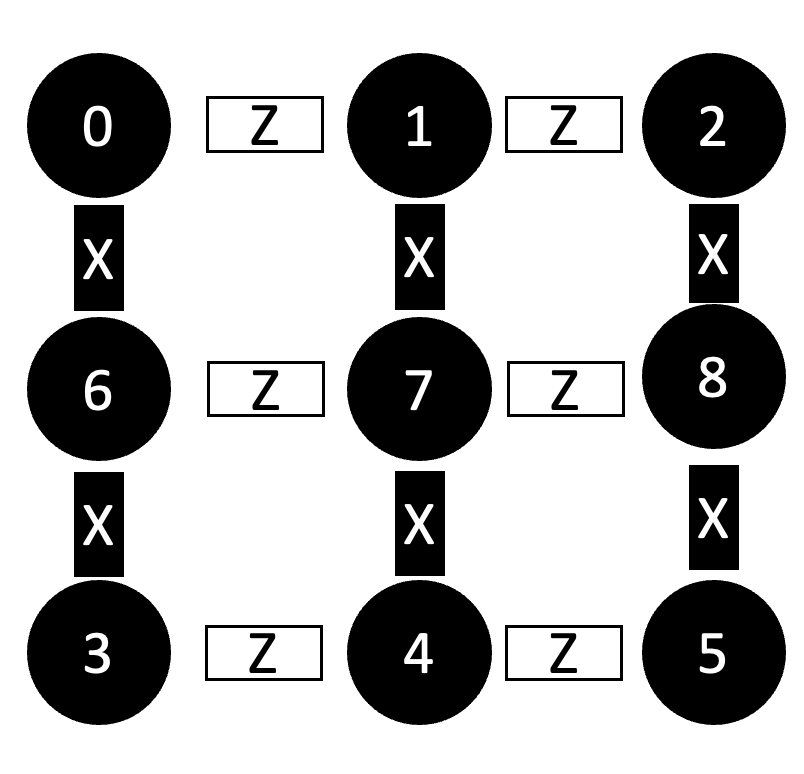
\includegraphics[scale=0.5]{baconshorcode.png}
\centering
\caption{A diagram of the Bacon Shor Code's gauge operators.}
\end{figure}


Algorithm \eqref{alg:euclid} was able to find the $\llbr 9,1,4,3 \rrbr $ Bacon Shor Code from the $ \llbr 9,1,3 \rrbr$ Shor code. This required first replacing two of the weight 2 $Z$ stabilizers with linearly independent weight 6 $Z$ stabilizers from the span of the weight 2 $Z$ stabilizers before running the Algorithm. Finding this quintessential subsystem code example with our algorithm points to its validity. We note here that although six gauge operators are shown in the diagram, not all are linearly independent. The last two are the product of the linearly independent gauge operators and a stabilizer. This technique can be generalized for other CSS concatenated codes. 


\subsection{$\llbr 9,1,2,2 \rrbr$ Rotated Surface Subsystem Code}



\begin{figure}[ht]
 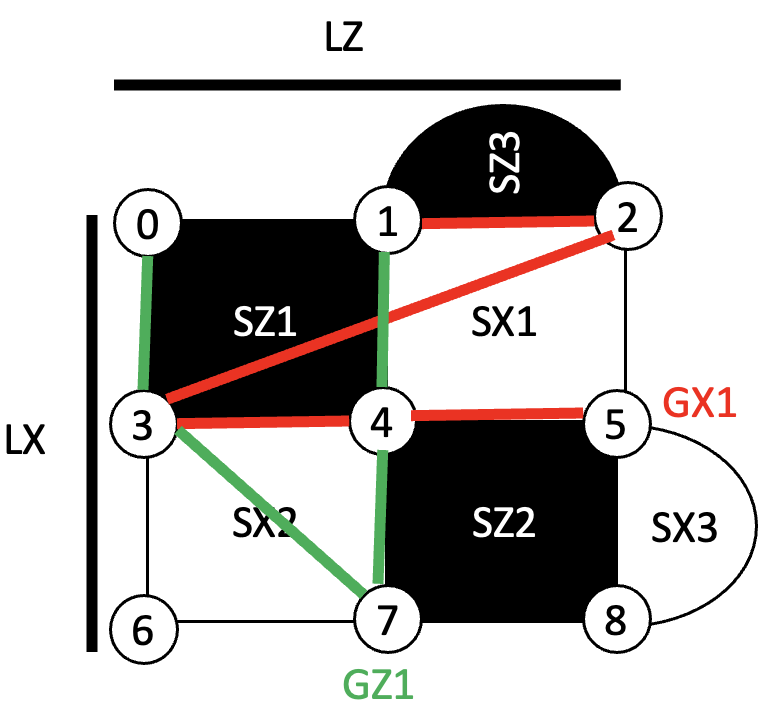
\includegraphics[scale=0.6]{surfacesubsystem1.png}
\centering
\caption{A diagram of the Rotated Surface Subsystem Code. The red operators are the $X$ gauge operators, and the green operators are $Z$. The product of the pair of red gauge operators gives $SX_{1}$, and the product of the pair of green operators gives $SZ_{2}$. Finding $SX_{2}$, $SZ_{2}$ can be done by multiplying $GX_{1}$, $GZ_{1}$ by the respective stabilizers to find the respective dependent gauges. ($GX_{2}$, $GZ_{2}$ are not shown here).}
\end{figure}
In this example, we show a novel subsystem version of the $\llbr 9,1,3 \rrbr$ rotated surface code found by Algorithm \eqref{alg:euclid}. Using the dependent gauges and gauge generators $GX_{1}$, $GZ_{1}$, we can measure all of the weight 4 stabilizers shown above at the cost of the dependent gauge operators being non-local and a small loss of distance. The other example we found in the literature of a subsystem version of a surface code had weight 6 stabilizers instead of the usual weight 4 \cite{higgott2021subsystem}. We summarize the set of gauge operators below: 


\begin{table}[H]
    \centering
    
    \begin{tabular}{c|c}
    \hline
 \multicolumn{2}{| c |}{List of $ \llbr 9,1,2,2 \rrbr$ subsystem code gauge operators}\\
 \hline
 Gauge Operator & Form\\
 \hline
 

    $GX_{1}$ & $X_{3}X_{4}X_{5}$ \\ 
     $GX_{2}$ & $X_{3}X_{4}X_{7}$\\ 
     $GX_{1d}$ & $X_{1}X_{2}X_{3}$\\ 
     $GX_{2d}$ & $X_{5}X_{6}X_{7}$\\ 
     $GZ_{1}$ & $Z_{1}Z_{4}Z_{7}$\\ 
     $GZ_{2}$ & $Z_{4}Z_{5}Z_{8}$\\ 
     $GZ_{1d}$& $Z_{0}Z_{3}Z_{7}$\\ 
     $GZ_{2d}$& $Z_{1}Z_{5}Z_{8}$  \\ \hline

    \end{tabular}
    \caption{Table of gauge operators in the gauge group of the $ \llbr 9,1,2,2 \rrbr$ rotated surface subsystem code }
    \label{tab:my_label}
\end{table}


\subsection{$\llbr 100,25,3 \rrbr$ Hypergraph Product Subsystem Code}



Using Algorithm \eqref{alg:euclid2}, we present a $\llbr 100,25,3 \rrbr$ SHP code built from a (10,5) linear block parity check matrix \cite{ryan2004introduction}: 
\begin{equation} \label{eq:H_binary} \boldsymbol{H}=
\begin{bmatrix}
    1&1&1&1&0&0&0&0&0&0 \\
    1&0&0&0&1&1&1&0&0&0 \\
    0&1&0&0&1&0&0&1&1&0 \\
    0&0&1&0&0&1&0&1&0&1\\
    0&0&0&1&0&0&1&0&1&1
\end{bmatrix}.
\end{equation}
We construct the SHP code with the following construction \cite{li2020numerical}:
\begin{align}
\label{eq:SHP}
\mathcal{G}_{X} &= \left(\boldsymbol{H}\otimes \boldsymbol{I}_{n}\right), \nonumber\\ 
\mathcal{G}_{Z} &= \left(\boldsymbol{I}_{n} \otimes \boldsymbol{H} \right), \nonumber\\ 
\mathcal{L}_{X} &= \left(\boldsymbol{I}_{n} \otimes \boldsymbol{G}\right),\\ 
\mathcal{L}_{Z} &= \left( \boldsymbol{G}\otimes \boldsymbol{I}_{n} \right), \nonumber\\ 
\mathcal{S}_{X} &= \left(\boldsymbol{H} \otimes \boldsymbol{G}\right), \nonumber\\ 
\mathcal{S}_{Z} &= \left( \boldsymbol{G}\otimes \boldsymbol{H}\right) \nonumber,
\end{align}
where $\boldsymbol{G}$ is the generator matrix of the code defined by the parity check matrix $\boldsymbol{H}$. $\boldsymbol{G}$ contains the basis for the linear code, and $\boldsymbol{G}\boldsymbol{H}^{T}=0$.
Thus, in general, the SHP construction in this form gives a $\llbr n^{2},k^{2},d \rrbr$ code with $n,k,d$ being the respective values for the classical code defined by the parity check matrix $\boldsymbol{H}$. Here, the key point is that although the stabilizers for this code are weight 12, our algorithm finds a decomposition that only requires weight $4$ operators with a residual weight of $0$ for the X stabilizers and weight $4$ operators with a residual weight of $5$ for the Z case. This is in contrast to the gauge operators which are all weight $4$ found from the closed-form expression in \eqref{eq:SHP}, requiring residual weights of $6$ and $16$ for X and Z stabilizers respectively. Thus, not only does our algorithm find more gauge operators than the closed-form expression, it also finds gauge operators that decompose the given stabilizers more efficiently than the closed-form operators. This decomposition makes this high-rate code far easier to implement. We also note that high-weight stabilizers are common for the SHP construction, as shown by the $ \llbr 49,16,3 \rrbr$ SHP code built from the [7,4,3] Hamming code with stabilizer weights 12 and 16, respectively. The parity check matrix for the [7,4,3] Hamming code is given below.  
\begin{equation} 
\label{eq:Hamm} 
\boldsymbol{H}=
\begin{bmatrix}
    1&1&1&0&1&0&0\\
    1&1&0&1&0&1&0\\
    1&0&1&1&0&0&1
\end{bmatrix}
\end{equation}

\subsection{Lifted-Product Subsystem Codes}
A natural extension of hypergraph product codes, lifted-product codes are constructed from the hypergraph product construction of parity check matrices $\boldsymbol{A}$ lifted over the ring $R=\mathbb{F}_{q}(G)$, where $G$ is some group. The construction of the parity check matrices then is as follows \cite{panteleev2021quantum}:
\begin{align}
\label{eq:LP}
\boldsymbol{H}_{X}=\left[ \boldsymbol{A} \otimes \boldsymbol{I}_{m_{A}}, \boldsymbol{I}_{m_{A}} \otimes \boldsymbol{A} \right ] \\
\boldsymbol{H}_{Z}=\left[ \boldsymbol{I}_{m_{A}} \otimes \boldsymbol{A}^{*},  \boldsymbol{A}^{*}\otimes \boldsymbol{I}_{m_{A}} \right ] 
\end{align}
where $\boldsymbol{A}^{*}$ is the conjugate transpose of $\boldsymbol{A}$. This construction is typically used with good LDPC codes, but whose sparsity ends up producing non-local stabilizer operators. When LDPC codes are placed into \eqref{eq:LP}, and are used as input for Algorithm 2, the algorithm is able to find several gauge operators for these codes. However, none of them are useful for our purposes since the resultant weight of the leftover gauges will greatly exceed the weight of the stabilizers themselves. This fact seems to stem from the sparse nature of the stabilizers themselves: in order to commute with them, the gauge operators must also be sparse, which in turn requires a larger amount of residual weight to cover the spread of the stabilizers. \\ 
\subsection{The SLP Construction}
To find a lifted code with a better gauge decomposition, one might be tempted to use the SHP construction in \eqref{eq:SHP} as a natural extension of Lifted Product Codes. We will refer to it as the SLP construction. Placing the base parity check matrix $\boldsymbol{H}$ along with its generator matrix  $\boldsymbol{G}$ into \eqref{eq:SHP} and then lifting the construction by a circulant size $L$ gives a   $\llbr Ln^{2},Lk^{2},D \rrbr$ code, where $n,k$ are the respective values defined by the base parity check matrix $\boldsymbol{H}$. Here $\boldsymbol{H}\boldsymbol{G}^*=0$, which implies that $\mathcal{G}_{X}\mathcal{S}^*_{Z}=0$. This lifting procedure yields codes with potentially larger distances than a typical SHP code. Let us now compare SHP with the SLP construction.
\subsubsection{Comparing the SHP and SLP Constructions}
For the most direct comparison, we choose a binary base matrix:
\begin{equation} 
\label{eq:Abinary} 
\boldsymbol{A}=
\begin{bmatrix}
    0&1&1\\
    1&1&0
\end{bmatrix},
\end{equation}
where the generator matrix of \eqref{eq:Abinary} is given by:
\begin{equation} 
\label{eq:Abinarygen}
\boldsymbol{G}_{\boldsymbol{A}}=
\begin{bmatrix}
    1&1&1
\end{bmatrix}.
\end{equation}
Placing into \eqref{eq:SHP}, this yields a $\llbr 9,1,3 \rrbr$ SHP code otherwise known as the Bacon-Shor Code, as discussed in Section V. A. For the SLP construction, we interpret \eqref{eq:Abinary} as the matrix of powers of monomials corresponding to $L=2$ circulant matrices. Thus we define our new base matrix as:
\begin{equation} 
\label{eq:Acirc} 
\boldsymbol{A}_{base}=
\begin{bmatrix}
    1&x&x\\
    x&x&1
\end{bmatrix}.
\end{equation}
Clearly \eqref{eq:Abinarygen} interpreted in the same fashion is no longer a valid solution, so we must use another generator matrix. It can be shown that the following matrix is a valid generator matrix for the base matrix code:
\begin{equation} 
\label{eq:Acirc} 
\boldsymbol{G}_{\boldsymbol{A}_{base}}=
\begin{bmatrix}
    1+x&0&1+x\\
\end{bmatrix}.
\end{equation}
This yields a  $\llbr 18,2,4 \rrbr$ SLP code. Although the rates of both the SHP and SLP codes are the same, the SLP code provides a larger distance. 
We now look at a few non-trivial examples of the SLP construction and their performance.

\subsubsection{$\llbr 27,12,3 \rrbr$ SLP code}



Given $L=3$, the $\llbr 27,12,3 \rrbr$ SLP code can be constructed by the following base parity check matrix:
\begin{equation} 
\label{eq:A_27} 
\boldsymbol{A}=
\begin{bmatrix}
    1+x+x^2&1+x&x
\end{bmatrix},
\end{equation}
along with the base generator matrix of the code:
\begin{equation} \label{eq:GA_27} \boldsymbol{G}_{\boldsymbol{A}}=
\begin{bmatrix}
   x^2&x&1\\
   x&x^2&x
\end{bmatrix}.  
\end{equation}

After inserting these into \eqref{eq:SHP} and lifting the construction, we find that the Pauli weight of the code's Stabilizers is 18, and the Pauli weight of the gauge operators is 6. We also find that the gauge operators in the closed-form construction decompose the stabilizers with a residual weight of 9, given three weight 6 gauge operators as input. However, our algorithm is able to decompose the stabilizers with residual weights of  4,6,8 for the $X$ and $Z$ stabilizers: an improvement over the closed-form gauge operator decomposition. Finally, we also note that the rate of the SLP construction is $\frac{4}{9}$, which is greater than the rate of the $ \left[\left[39,12,3\right]\right]$  LP code constructed from the same base matrix, $\frac{4}{13}$. This is also while preserving the same distance between codes. 
\subsubsection{$\llbr 775,124,62 \rrbr$ SLP code}
For our final example, we give the SLP code constructed by Tanner's (3,5) QC-LDPC code with $L$=31. Here, we use the following base matrix \cite{raveendran2022finite}:


\begin{equation} 
\label{eq:B31} 
\boldsymbol{B}=
\begin{bmatrix}
    x&x^{2}&x^{4}&x^{8}&x^{16}\\
    x^{5}&x^{10}&x^{20}&x^{9}&x^{18}\\
    x^{25}&x^{19}&x^{7}&x^{14}&x^{28}
\end{bmatrix}. 
\end{equation}
As shown by Chimal-Dzul, Lieb, and Rosenthal \cite{chimal2022generator}, a generator matrix for \eqref{eq:B31} can be constructed in the following way:
\begin{equation} \label{eq:G31} \boldsymbol{\mathcal{G}}=
\begin{bmatrix}
    u_{11}&u_{12}&u_{13}&u_{14}&0\\
    u_{21}&u_{22}&u_{23}&0&u_{25}\\
    f&f&0&0&0\\
    f&0&f&0&0\\
    f&0&0&f&0\\
     f&0&0&0&f
\end{bmatrix},
\end{equation}


   

\begin{flalign}
\label{eq:partsofGfull31}
u_{11} = x^{28} + x^{25} + x^{18} + x^{16} + x^{5} + x,\\
u_{12} = x^{23} + x^{22} + x^{20} + x^{17} + x^{7} + x^{4},\nonumber\\
u_{13} = x^{29} + x^{25} + x^{21} + x^{12} + x^{5} + x,\nonumber\\
u_{14}= u_{25} = x^{28} + x^{18} + x^{16} + x^{14} + x^{9} + x^{8},\nonumber\\
u_{21} = x^{27} + x^{24} + x^{19} + x^{11} + x^{10} + x^{2},\nonumber\\
u_{22} = x^{30} + x^{28} + x^{26} + x^{18} + x^{16} + x^{6},\nonumber\\
u_{23} = x^{20} + x^{14} + x^{9} + x^{8} + x^{7} + x^{4},\nonumber\\
f=\frac{x^{31}-1}{x-1}=x^{30} + \cdots + x + 1.\nonumber
\end{flalign}
Taking rows 3,4 we form our generator matrix for the code:
\begin{equation} 
\label{eq:G31} 
\boldsymbol{G}_{\boldsymbol{B}}=
\begin{bmatrix}
    f&f&0&0&0\\
    f&0&f&0&0
\end{bmatrix},
\end{equation}
we find that the code has stabilizer weights of 310 and gauge operator weights of 5. Due to the large number of physical qubits, this code is beyond the practical scale that our algorithm can handle. Our algorithm is suited for small to medium-sized codes due to its exponential memory complexity, but this decomposition by GNarsil may be achievable with a sufficiently large amount of memory. However, we were able to use a sub-gradient descent solver, which finds the coordinate vector $\boldsymbol{x}$ that minimizes $\left|\left|\boldsymbol{G}\boldsymbol{x}-\boldsymbol{s}\right|\right|$, to find splits. Here, $\boldsymbol{G}$ is the matrix of possible gauge operators, and $\boldsymbol{s}$ is the vector representing the stabilizer. The solver found splits with residual weight of around 230, using approximately 100 weight 5 gauge operators. It is unknown whether this solution is optimal or not. Our SLP example demonstrates that the SLP construction can be quite advantageous if a generator matrix can be found for a certain base matrix. For the same matrix \eqref{eq:B31}, an LP($\boldsymbol{B}$,$\boldsymbol{B}^*$) construction yields a $\llbr 1054,124,20 \rrbr$ code, which trails the SLP version both in rate and in distance. If a circulant form generator matrix is found for a Base Matrix, the resulting SLP code will have a higher rate than its Lifted Product counterpart with the same dimension code space. No relationship between the distance of the two constructions has been formalized, but it seems that the SLP code will at least have the same distance as its Lifted Product counterpart. 
This makes the SLP construction for a given base matrix, when possible, a very attractive construction. 



\section{Conclusion}
In this paper, we have introduced a new set of algorithms we call GNarsil for finding subsystem codes with gauge operators that compose up to a stabilizer. We have demonstrated that these algorithms can find not only well-known examples of subsystem codes but also novel ones, such as a novel Hypergraph Product Subsystem code, that surpasses the residual weight decomposition performance of the closed-form structure of the subsystem version of this code and novel version of the Surface code. We also show that we could not find useful decompositions of Lifted Product codes due to the highly non-local structure of the stabilizers, but by using the SLP construction, we can find codes that have fair decomposition properties that our algorithm can improve, but also excellent rate and distance. As noted, this also depends on finding a generator matrix for the base matrix in circulant form, which is not guaranteed to always exist.  We foresee these algorithms becoming a useful tool for finding subsystem versions of stabilizer codes that may prove easier to implement due to the stabilizers' decomposition into smaller weight gauge operators. However, it is clear that this problem remains complex, as the solution spaces for useful gauge generators are sparse, making it likely that our algorithms are optimal for this case, even though they are exponentially complex in memory. Thus our algorithms work best for small to medium-sized codes. Improving our algorithm's performance will most likely require specializing it for a certain type of code construction. This would allow us to exploit symmetries of certain codes to find optimal gauge operators. We also foresee that the measure of residual weight can be useful for understanding the properties of good subsystem codes and what symmetries they may possess. Finally, we wish to extend this work into looking at the relationship between fault-tolerant operations on a stabilizer code and its related subsystem code by extending tools such as the LCS algorithm 
 by seeing how new gauge operators found by our algorithm change the structure of logical gates for our code from the stabilizer seed code to the new subsystem version of it.\cite{rengaswamy2018synthesis}. Insights into this relationship may be useful for the development of Floquet codes. \\
 \section*{Acknowledgements}
 We thank Nithin Raveendran and Bane Vasić at the University of Arizona for their insights into Lifted-Product and QC-LDPC codes, respectively. We would also like to thank them for their insights into finding circulant form generator matrices for QC-LDPC codes. Finally, we would also like to thank Muhammad Sohaib Alam at the Universities Space Research Association for his insights into subsystem codes and the workings of our algorithm. 

 \section*{Appendix A: Proof of Algorithm's Ability to find all possible representations of a subsystem code using Binary Symplectic Matrices. }
\begin{theorem} Given an $\left[[n,k,d]\right]$ code with logical operators $\boldsymbol{X_{i}},\boldsymbol{Z_{i}}$  for each logical qubit, the algorithm can find all representations for the $2r$ gauge generators of an $\left[[n,k,r,d]\right]$ subsystem code, where $2n-2r$ of the rows of the code are fixed.

\begin{proof}
Let $r$ be the number of gauge qubits chosen from the input code. The input code is described by a $2n \times 2n$ matrix $\boldsymbol{U}$, a symplectic matrix that describes the code's logical operators, and stabilizers. The row vectors $\langle\boldsymbol{u}_{1},...,\boldsymbol{u}_{2n}\rangle \in \mathbb{F}^{2n}_{2}$ of $\boldsymbol{U}$ then span the space $\mathcal{U}	= \mathbb{F}^{2n}_{2}$. We choose $2r$ vectors $\langle \boldsymbol{u}_i : i\in \mathcal{I}\rangle_{}$,  $\mathcal{I}=\langle I_{1},I_{1}+r,...,I_{r},I_{r}+r\rangle, I_{k}\in \langle 1,...,2n-r \rangle$ from $\boldsymbol{U}$ which correspond to a submatrix of  $\boldsymbol{U}$,  $\boldsymbol{U}_r$. These vectors from $\mathcal{I}$ form a symplectic basis for a $2^{2r}$ dimensional subspace $\mathcal{U}_{r} \subseteq \mathcal{U}$.
Since the subspace is symplectic, we see that any vector $\boldsymbol{u}_{i}, i\in \mathcal{I}$ has a symplectic product with any vector $\boldsymbol{u}_{j}, j\notin \mathcal{I}$,  $\langle \boldsymbol{u}_{i},\boldsymbol{u}_{j}\rangle_{s}=0 $ (mod 2). \\ We now replace the vectors from  $\boldsymbol{U}_r$ with vectors  $\tilde{\boldsymbol{u}}=\langle \boldsymbol{u}_{i},\boldsymbol{u}_{j} \in \mathcal{U}_r : i,j \notin \mathcal{I}, \langle\boldsymbol{u}_{i},\boldsymbol{u}_{i+r}\rangle_{s}=\langle\boldsymbol{u}_{j},\boldsymbol{u}_{j+r}\rangle_{s} =1$ (mod 2)$\rangle$. To see which pairs of vectors in $\mathcal{U}_r$ form valid symplectic pairs we arrange all of the symplectic products of vectors in $\mathcal{U}_r$ into a matrix $\boldsymbol{P}=\sum_{ij} \langle \boldsymbol{u'}_{i},\boldsymbol{u'}_{j}\rangle_{s}\ket{i}\bra{j} $ (mod 2) where $\boldsymbol{u'}_{i},\boldsymbol{u'}_{j} \in \mathcal{U}_r$. 
We use $\boldsymbol{P}$ to count the number of possible representations generated of symplectic pairs of $\mathcal{U}_{r}$. The number of representations is defined as the number of unique matrices $\boldsymbol{V}$ built from $\boldsymbol{U}$ by replacing the vectors $\langle \boldsymbol{u}_i : i\in \mathcal{I}\rangle_{}$ with  vectors in $\tilde{\boldsymbol{u}}$  such that $\boldsymbol{V}\boldsymbol{\Omega}\boldsymbol{V}^T=\boldsymbol{\Omega}$, where $\boldsymbol{\Omega}=\begin{bmatrix} 
  \boldsymbol{0} & \boldsymbol{I}_n \\
  \boldsymbol{I}_n & \boldsymbol{0}
  \end{bmatrix}$
  
   This condition is equivalent to all constraints needed to be satisfied by a valid subsystem code. The number of representations for a given $r$ can be found by examining $\boldsymbol{P}$. For instance, in the case of $r=2$ we see that:
       
  \begin{equation}\boldsymbol{P}=\begin{bmatrix}
  \begin{smallmatrix}
       0 & 0 & 0 & 0 & 0 & 0 & 0 & 0 & 0 & 0 & 0 & 0 & 0 & 0 & 0 & 0\\
       0 & 0 & 0 & 0 & 1 & 1 & 1 & 1 & 0 & 0 & 0 & 0 & 1 & 1 & 1 & 1\\
       0 & 0 & 0 & 0 & 0 & 0 & 0 & 0 & 1 & 1 & 1 & 1 & 1 & 1 & 1 & 1\\
       0 & 0 & 0 & 0 & 1 & 1 & 1 & 1 & 1 & 1 & 1 & 1 & 0 & 0 & 0 & 0\\
       0 & 1 & 0 & 1 & 0 & 1 & 0 & 1 & 0 & 1 & 0 & 1 & 0 & 1 & 0 & 1\\
       0 & 1 & 0 & 1 & 1 & 0 & 1 & 0 & 0 & 1 & 0 & 1 & 1 & 0 & 1 & 0\\
       0 & 1 & 0 & 1 & 0 & 1 & 0 & 1 & 1 & 0 & 1 & 0 & 1 & 0 & 1 & 0\\
       0 & 1 & 0 & 1 & 1 & 0 & 1 & 0 & 1 & 0 & 1 & 0 & 0 & 1 & 0 & 1\\
       0 & 0 & 1 & 1 & 0 & 0 & 1 & 1 & 0 & 0 & 1 & 1 & 0 & 0 & 1 & 1\\
       0 & 0 & 1 & 1 & 1 & 1 & 0 & 0 & 0 & 0 & 1 & 1 & 1 & 1 & 0 & 0\\
       0 & 0 & 1 & 1 & 0 & 0 & 1 & 1 & 1 & 1 & 0 & 0 & 1 & 1 & 0 & 0\\
       0 & 0 & 1 & 1 & 1 & 1 & 0 & 0 & 1 & 1 & 0 & 0 & 0 & 0 & 1 & 1\\
       0 & 1 & 1 & 0 & 0 & 1 & 1 & 0 & 0 & 1 & 1 & 0 & 0 & 1 & 1 & 0\\
       0 & 1 & 1 & 0 & 1 & 0 & 0 & 1 & 0 & 1 & 1 & 0 & 1 & 0 & 0 & 1\\
       0 & 1 & 1 & 0 & 0 & 1 & 1 & 0 & 1 & 0 & 0 & 1 & 1 & 0 & 0 & 1\\
       0 & 1 & 1 & 0 & 1 & 0 & 0 & 1 & 1 & 0 & 0 & 1 & 0 & 1 & 1 & 0   
   \end{smallmatrix}
   \end{bmatrix}\end{equation}
    By examining $\boldsymbol{P}$, we first see that there are $15$ vectors of $\mathcal{U}_r$ that can form a sympletic pair or $2^{2r}-1, r=2$. Each of those vectors has $8$ available symplectic partners, or $2^{2r-1}, r=2$ possible partners. For finding the third vector to put into $\boldsymbol{V}$ out of $2r, r=2$ needed vectors, and we look for possible candidates by searching for the columns corresponding to the vectors where the first two vectors' rows in $\boldsymbol{P}$ are $0$. We find $4$ such columns but note that one is the column corresponding to the trivial vector or column $1$. We, therefore, have $3$ possible nontrivial choices for the third vector or $2^{2r-2}-1, r=2$ possible choices. Finally, we search the compatible symplectic pairs of the third vector where the first two vectors' rows are zero. This gives us $2$ choices or $2^{2r-3},r=2$. Thus, our total number of subsystem codes for $r=2$ is $720$. However, this number includes the multiplicity of codes due to the possible permutations of the $2r$ rows that still allow $\boldsymbol{V}$ to satisfy  $\boldsymbol{V}\boldsymbol{\Omega}\boldsymbol{V}^T=\boldsymbol{\Omega}$. By looking at all possible permutations of the rows such that we preserve the symplectic pairs between the row vectors, we find that the multiplicity is $8$ for $r=2$. Thus, the total number of unique representations for $r=2$ is $90$. We can extrapolate this procedure to arbitrary $r$ and find that the number of representations for a given $r$ is:
\begin{equation} 
N_{sub}(r)=\frac{\left( \prod_{l\in\left( 0,2 \right), r\geq 2} 2^{2r-l}-1\right)\left(\prod_{m\in\left(1,3,4,...,2r-1\right)}2^{2r-m}\right)}{\mathcal{M}},\\
 \end{equation} 
 where $\mathcal{M}$ is the multiplicity of the $2r$ rows.\\

   
Finally, we denote the set of possible representations by $\mathcal{R}$. Let us assume that there exists a representation in $\mathcal{R}$ built out of our starting matrix $\boldsymbol{U}$, fixing its vectors which are not those with indices in $\mathcal{I}$, and whose gauge operators either come from $\mathcal{U}_r$ but were not counted by the algorithm as a valid subsystem code or whose gauge operators are not from $\mathcal{U}_r$. These vectors were not counted for the first case because they do not form symplectic pairs. Therefore, the representation code is not valid. In the second case, since $\boldsymbol{U}$ spans $\mathbb{F}^{2n}_{2}$, the gauge operators must be linear combinations of the vectors of $\langle \boldsymbol{u}_i, i\notin \mathcal{I} \rangle$. Thus, the representation is invalid since its matrix is linearly dependent. Therefore, the algorithm can find all valid representations of a subsystem code given a fixed set of $2n-2r$ vectors.  
    \end{proof}
    \end{theorem}

\bibliographystyle{IEEEtran}
\bibliography{cites} 


\end{document} 
